\documentclass[letterpaper,10pt,draftclsnofoot,onecolumn,titlepage]{IEEEtran}

\usepackage{graphicx}
\usepackage{amssymb}
\usepackage{amsmath}
\usepackage{amsthm}
\usepackage{alltt}
\usepackage{float}
\usepackage{color}
\usepackage{url}
\usepackage{enumitem}
\usepackage{pstricks, pst-node}
\usepackage{geometry}
\usepackage{array}
\usepackage{listings}
\usepackage{caption}
\usepackage{subcaption}
\usepackage{import}
\usepackage[final]{pdfpages}

\renewcommand{\lstlistingname}{Code}

\geometry{margin = .75in}

\usepackage{hyperref}

\usepackage[acronym]{glossaries}

\makeglossaries

\newglossaryentry{iOS}{name={iOS}, description={A mobile operating system created and developed by Apple Inc. exclusively for Apple's hardware}}
\newglossaryentry{ModelVC}{name={Model-View-Controller}, description={A design pattern that assigns objects in an application one of three roles: model, view, or controller. Also called MVC}}
\newglossaryentry{Android}{name={Android}, description={A mobile operating system developed by Google, based on the Linux Kernel and designed primarily for touchscreen mobile devices}}
\newglossaryentry{App}{name={app}, description={A software application designed to run on mobile devices such as smartphones or tablet computers}}
\newacronym{ccb}{CCB}{Church Community Builder}
\newacronym{sdd}{SDD}{Software Design Document}
\newacronym{srs}{SRS}{Software Requirements Specification}
\newacronym{uml}{UML}{Unified Model Language}
\newacronym{mvc}{MVC}{Model-View-Controller}
\newacronym{xml}{XML}{EXtensible Markup Language}
\newacronym{ui}{UI}{User Interface}




\graphicspath{{figures/}{pictures/}{images/}{./}}


\newcommand*{\signature}[1]{%
	\par\noindent\makebox[3.5in]{\hrulefill} \hfill\makebox[3.0in]{\hrulefill}%
	\par\noindent\makebox[3.5in][l]{#1}	    \hfill\makebox[3.0in][l]{Date}%
}%

\def\name{Kevin Stine, Courtney Bonn, Maxwell Dimm}
\def\team{Calvary Chapel Corvallis}
\def\grp{Group \#62}

\hypersetup{
	colorlinks = true,
	urlcolor = black,
	linkcolor = black,
	pdfauthor = {\name},
	pdftitle = {CS463 Final Report},
	pdfsubject = {CS463 Final Report},
	pdfpagemode = UseNone
}

\begin{document}
	\title{\huge \team \\ Final Report\\ CS 463 Spring 2017}
	\author{\large \name \\ \grp}



	\maketitle

		\begin{abstract}The purpose of this project is to produce an \gls{iOS}/\gls{Android} application for Calvary Chapel of Corvallis that will allow members to access a plethora of information all in one localized space.
		The Church's current website does not provide an interface where current members of the church can very quickly access important information such as events, bulletins, and messages from the service.
		The desired application will be simple enough for anyone to use while providing back end access for staff to easily upload new information to the app.
		The priorities lie in maximizing the usability of the app and providing bulletin, schedule, video, and giving functionality.
		We will work with the existing Calvary Chapel web development team to create a product that is seamlessly integrated with their already existing network.
		\end{abstract}

		\clearpage

		\tableofcontents

		\clearpage

\section{Introduction}

Our project centered around a local church in Corvallis, Oregon, Calvary Chapel of Corvallis.
The church requested our help in creating a mobile application that would work together with their existing website and be used by the members of the congregation.
Our main goal was to create an application that was compatible with both iOS and Android smart phones, had a simple design and functionality so all people could use it easily, and incorporated the most important pieces of their current website.
It was decided that the main sections the church wanted to see on the applications were the bulletins, events, the ability to donate, and the most recent message video.

The client team was led by project manager, Desiree Gorham.
She acted as a channel of communication between us and the senior staff at the church to make sure we were designing the app in the way they had intended.
The church was not involved in development, but did offer advice and ideas as to how they wanted the final product to look and function.

The members of our team were Courtney Bonn, Maxwell Dimm, and Kevin Stine.
The project requirements were spread among us, though we did change those assignments throughout the process as well as helped each other when needed.
The roles were as follows:

\begin{itemize}
	\item Courtney Bonn: iOS - Bulletin Page; Android - Bulletin, Donation, Events Page
	\item Max Dimm: iOS - Donation, Messages Page; Android - Messages Page
	\item Kevin Stine: iOS - Events Page
\end{itemize}

\section{Original Requirements}

	\includepdf[pages={2-8}]{originals/requirements.pdf}

\section{Requirement Changes}

\section{Original Design Document}

	\includepdf[pages={2-12}]{originals/design.pdf}

	\subsection{Design Changes}

\section{Original Technology Review}

	\includepdf[pages={2-23}]{originals/tech-review.pdf}

	\subsection{Technology Changes}
	Throughout the process of building our applications, the church was also busy working on their own website.
	The new church website used Wordpress as the software backing the entire site.
	Because we wanted to limit the amount of extra work required to maintain the application, it made sense to change the way we were incorporating the bulletin page into the app.

	Originally, we proposed to incorporate the bulletin page using the database, \gls{ccb}.
	The bulletin announcements were going to be handled in this database, which we could then request through the API.
	However, with the new website, the bulletins were no longer going to be updated on the database.
	This meant, should we choose to use this database, the church would have to update the database as well as the website in order to update the app.

	Because their new website used Wordpress, we were able to make use of the Wordpress REST API.
	By utilizing this API, we could request the content on the bulletin page and using a JSON parser, we could display the results on the application.
	Now, whenever the website updates, the app will update as well.

	There were no other technology changes.

\section{Weekly Blog Posts}

	\import{./}{blogposts}

\section{Final Poster}

\includepdf[pages={-}]{originals/poster.pdf}

\section{Project Documentation}

Our project works in two different ways, depending on it is begin ran as a developer or as a consumer.
Because the end result is an application, available on both iOS and Android platforms, the project's structure is very simple.
There are two sets of project files, one for each platform, and within the files the code that can be executed in order to run the application is available.

As a consumer, one can download the application from the app store once it has been published.
After downloading, it will be available to use on the corresponding phone.
The app itself takes up less than 40 MB of space on a phone.

As a developer, the applications can be ran on a computer using two different softwares: Xcode and Android Studio.
These softwares are required in order to run the code.
They can be downloaded from \url{https://developer.apple.com/xcode/} or \url{https://developer.android.com/studio/index.html}.
One caveat, though, is that to be eligible to download Xcode, one must be on a Mac computer.
Android Studio can be downloaded from both Mac and Windows computers.

Once the required software is installed, the code can be downloaded from \url{https://github.com/ikaikastine/capstone-group-62} with the code living in the folders iOS and Android.
The projects can then be opened in the corresponding software and ran accordingly.
The software allows one to run the code on either a built in simulator or an actual device if it is connected to the computer.



\section{Learning New Technology}
Because mobile development was new to all of us, we had to spend a good portion of our time researching and becoming accustomed to using the mobile development software, Xcode and Android Studio.
The main sources which we used to learn these platforms, were produced by Apple and Android Studio.
Apple had a website in which it walked us through how to begin developing an iOS App on Xcode.
It taught us how to develop in Swift as well as how to use the program \cite{AppleSwift}.
Android Studio had a similar website, as well as sample apps we could walk through designing \cite{AndroidStudio}.

Besides learning the main platforms, we had to do a copious amount of research on how to implement each part of the app.
A website that was instrumental in learning how to parse the Wordpress pages into JSON objects and display the JSON response was Grok Swift \cite{JSONSwift}. Because we also needed to know how to handle JSON in Android, a thread on Stackoverflow was very helpful \cite{JSONAndroid}.

A tutorial on \url{www.androidbegin.com} was used to understand how to handle XML parsing and displaying the data on an Android app \cite{XMLAndroid}.
We needed this information to handle the events calendar through \gls{ccb}.

While there were other websites that we searched and read, the above websites were the most helpful in learning the new technology.
As far as print documentation, we did not utilize any reference books in our learning.
Our assigned teacher's assistant, Vedanth, did provide some suggestions to help us with our learning, as he had some experience in mobile development from his own senior project.

For the iOS Events page, a lot of time was spent looking at the Apple Developer API reference at \url{developer.apple.com/reference} to get familiar with the references for various portions of the application.
For the Events page specifically there was a lot of time spent looking at the DateFormatter reference, the NSDate reference, and UIDatePicker reference.
In addition to utilizing the developer API reference, Stack Overflow at \url{stackoverflow.com} was pretty critical in helping with debugging the code.
I found a lot of discrepancies between Swift 3.0 and older versions, so when my code had a bug, it was tough to find specific help related to that version of swift.
However I think that stackoverflow was instrumental in my success in debugging and with adding certain features like the UIDatePicker that utilized a particular type of object with the toolbar.

\section{Team Reflection}

	\subsection{Courtney Bonn}

		Because I had no worked with mobile development before I decided to choose this project, I was given the opportunity to learn an abundance of technical information.
		I went into this project with little understanding as to how an app worked and how to create my own.
		Fast forward to the end of the year and I know feel comfortable developing in both iOS and Android platforms, a skillset I am excited to get to add to my resume.
		Specifically, I learned how to code in Swift and brushed up on my Java language skills.
		I learned two new platforms to code in, Xcode and Android Studio.
		I also learned how to work with a REST API and JSON objects, as well as XML parsing and responses.
		Finally, I learned the whole process of creating an app from start to finish.

		The main non-technical bit of information that I learned this year was how to produce accurate and helpful documentation for a large project.
		While documentation can feel time-consuming, it ends up saving a lot of time because there is already a roadmap for the project.
		Beginning development with no documentation would have felt overwhelming and chaotic and more likely than not would have caused development to take at least twice the amount of time.
		Knowing how to produce the necessary documentation is something I am very grateful to have learned in this course.

		Until this class, most assignments I had worked on were weekly assignments, with a few term projects here and there.
		Even then, term projects did not usually take up the entire term, but perhaps the last couple of weeks.
		I have never experienced working on the same project for a year before.
		Learning to keep focus and interest in a project for this amount of time, was a valuable skill that I am taking away from this project.


		The biggest lesson I learned about project management, was that it is very easy to fall behind in a project if you go even one week without working on it.
		There were times where I could not work on the project for whatever reason, and then I felt I was behind in where I should be in project progression.
		The lesson I will take away is that even putting an hour into the project every week or a few minutes a day will help keep the project going smoothly.

		In my college career, I have worked in many group projects.
		More often than not, these projects lasted a few weeks to a term at most, and then we went our separate ways.
		To work with the same group for almost an entire year was a new experience for me and one that I enjoyed.
		I learned that you have to help one another because you have to work as a time--you cannot leave anyone behind.
		I also learned that you have to be patient with each other because not everyone is going to be able to commit the same amount of time or effort at all times.
		Because we all had different classes to focus on as well, we had to work together to make sure our project was not falling behind if we needed to work on other classes.


	\subsection{Max Dimm}

	\subsection{Kevin Stine}


	\bibliographystyle{IEEEtran}
	\bibliography{IEEEabrv,finalreport}

	\appendices

	\section{Essential Code Listings}

	\begin{lstlisting}[caption=iOS EventViewController Snippet]
func createDatePicker() {
    // format the picker
    datePicker.datePickerMode = UIDatePickerMode.date
    //toolbar
    let toolbar = UIToolbar()
    toolbar.sizeToFit()
    // bar button item
    let doneButton = UIBarButtonItem(barButtonSystemItem:
			.done, target: nil, action: #selector(donePressed))
    toolbar.setItems([doneButton], animated: false)
    changeDate.inputAccessoryView = toolbar
    changeDate.inputView = datePicker
}
\end{lstlisting}

This code creates the datePicker which allows the user to select the month, day and year.

\begin{lstlisting}[caption=iOS EventViewController Snippet]
func donePressed() {
    // format date
    let dateFormatter = DateFormatter()
    dateFormatter.dateFormat = "yyyy-MM-dd"
    pickerTracker = true
    startDate = dateFormatter.string(from: datePicker.date)
    updateTable()
    self.view.endEditing(true)
}
\end{lstlisting}

This code is the selected action for the DatePicker.

\begin{lstlisting}[caption=Android XML Parser]
 public String getXmlFromUrl(String url) {
       OkHttpClient client = new OkHttpClient();
           final String basic = "Basic " + Base64.encodeToString(CREDENTIALS.getBytes(),
           Base64.NO_WRAP);
           String str = null;
           Request request = new Request.Builder()
                   .url(url)
                   .header("Authorization", basic)
                   .build();

           try {
               Response response = client.newCall(request).execute();
               str = response.body().string();
           } catch (IOException e) {
               e.printStackTrace();
           }

       return str;
   }
\end{lstlisting}

\begin{lstlisting}[caption=iOS JSON Response]

{
  "id": 1038,
  "date": "2016-10-27T19:22:53",
  "date_gmt": "2016-10-27T19:22:53",
  "guid": {
    "rendered": "http://www.calvarycorvallis.org/?page_id=1038"
  },
  "modified": "2017-03-18T11:48:50",
  "modified_gmt": "2017-03-18T18:48:50",
  "slug": "bulletin",
  "status": "publish",
  "type": "page",
  "link": "https://www.calvarycorvallis.org/bulletin/",
  "title": {
    "rendered": "This Week&#8217;s Bulletin"
  },
  "content": {
    "rendered": "<p>all bulletin content would be here...
    ...
    },
    Additional, unrelated JSON returned below here...
 }

\end{lstlisting}

\begin{lstlisting}[caption=iOS JSON Parser]
 do {
 	guard let bulletin = try JSONSerialization.jsonObject(with: responseData,
	options: []) as? [String: AnyObject] else {
	         print("error trying to convert data to JSON")
                 return
         }

        	guard let bulletinContent = bulletin["content"]?["rendered"] as?
	String else {
                  print("Could not get bulletin content from JSON")
                  return
         }
         let actualContent = bulletinContent.replacingOccurrences(of: "<[^>]*.", with:
         "", options: .regularExpression, range: nil)

         DispatchQueue.main.async{
 	          self.jsontext.text = actualContent
         }
} catch  {
         print("error trying to convert data to JSON")
         return
}
\end{lstlisting}

\begin{lstlisting}[caption=Android JSON Parser]
if (response != null) {
	try {
		JSONObject jsonResponse = response.getJSONObject(TAG_CONTENT);
                 String jsonData = jsonResponse.getString(TAG_RENDERED);
		 textView.setText(jsonData);
                  Log.e("App", "Success: " + response.getString("yourJsonElement"));
	} catch (JSONException ex) {
                    Log.e("App", "Failure", ex);
        }
}
\end{lstlisting}

\begin{lstlisting}[caption=iOS Load into WebView]
let htmlCode = "<!DOCTYPE HTML><html><head><style> body {color: #5b5e5e; font-family:
'Lora', Palatino;} a { border-bottom: 1px solid #fbaf17; color: #fbaf17;
text-decoration: none; }
.staff a { border-bottom: 0px none; } a:focus, a:hover { border-bottom: 1px solid #fbaf17;
color: #b17b0e; }</style></head><body>" + bulletinContent + "</body></html>"

self.bulletinWeb.loadHTMLString(htmlCode, baseURL: nil)
		\end{lstlisting}

\begin{lstlisting}[caption=Android Load into WebView]
String bulletinContent = "<!DOCTYPE HTML><html><head><style> body {color: #5b5e5e;
font-family: 'Lora', Palatino;} a { border-bottom: 1px solid #fbaf17; color: #fbaf17;
text-decoration: none; } .staff a { border-bottom: 0px none; } a:focus, a:hover {
border-bottom: 1px solid #fbaf17; color: #b17b0e; }</style></head><body>" +
jsonData + "</body></html>";

myWebView.loadDataWithBaseURL("file:///android_asset/", bulletinContent,
"text/html", "utf-8", null);
myWebView.getSettings().setAllowFileAccess(true);
\end{lstlisting}


\begin{lstlisting}[caption=iOS Donation Page]
 	let donateURL = URL (string: "https://www.calvarycorvallis.org/give/")
        let requestObj = URLRequest(url: donateURL!)
        donateView.loadRequest(requestObj)
        donateView.delegate = self
        donateView.scrollView.delegate = self
        donateView.scrollView.isScrollEnabled = false
\end{lstlisting}

\begin{lstlisting}[caption=Android Donation Page]
@Override
    public void onPageFinished(WebView view, String url) {
            myWebView.loadUrl("javascript:(function() { " +
            "document.getElementsByClassName('site-header')[0].style.display='none'; " +
            "document.getElementsByClassName('footer-widgets')[0].style.display='none'; " +
            "document.getElementsByClassName('content')[0].style.display='none'; " + "})()");
            myWebView.setVisibility(View.VISIBLE);
            myWebView.getSettings().setLoadWithOverviewMode(true);
            myWebView.getSettings().setUseWideViewPort(true);
   	}
   });
        myWebView.setVisibility(View.GONE);
        myWebView.loadUrl("https://www.calvarycorvallis.org/give/");
\end{lstlisting}

\begin{lstlisting}[caption=Android Messages Page]
public View onCreateView(LayoutInflater inflater, ViewGroup container,
Bundle savedInstanceState) {
        myView = inflater.inflate(R.layout.fourth_layout, container, false);

        String videoLink = "<html><iframe id=\"ls_embed_1493363421\" src=\"
        https://livestream.com/accounts/18343788/events/7279945/videos/154327352/player
        ?width=960&height=540&enableInfo=false&defaultDrawer=&autoPlay=true&
        mute=false\" width=\"960\" height=\"540\" frameborder=\"0\" scrolling=\"no\"
        allowfullscreen> </iframe></html>";

        myWebView = (WebView) myView.findViewById(R.id.messagesView);

        WebSettings webSettings = myWebView.getSettings();
        webSettings.setJavaScriptEnabled(true);
        myWebView.getSettings().setLoadWithOverviewMode(true);
        myWebView.getSettings().setUseWideViewPort(true);
        myWebView.getSettings().setBuiltInZoomControls(true);
        myWebView.loadData(videoLink, "text/html", "utf-8");

        return myView;
		\end{lstlisting}


	\section{Photos}

	\begin{figure}[H]
			\centering
			\begin{subfigure}{.5\textwidth}
 				 \centering
  				 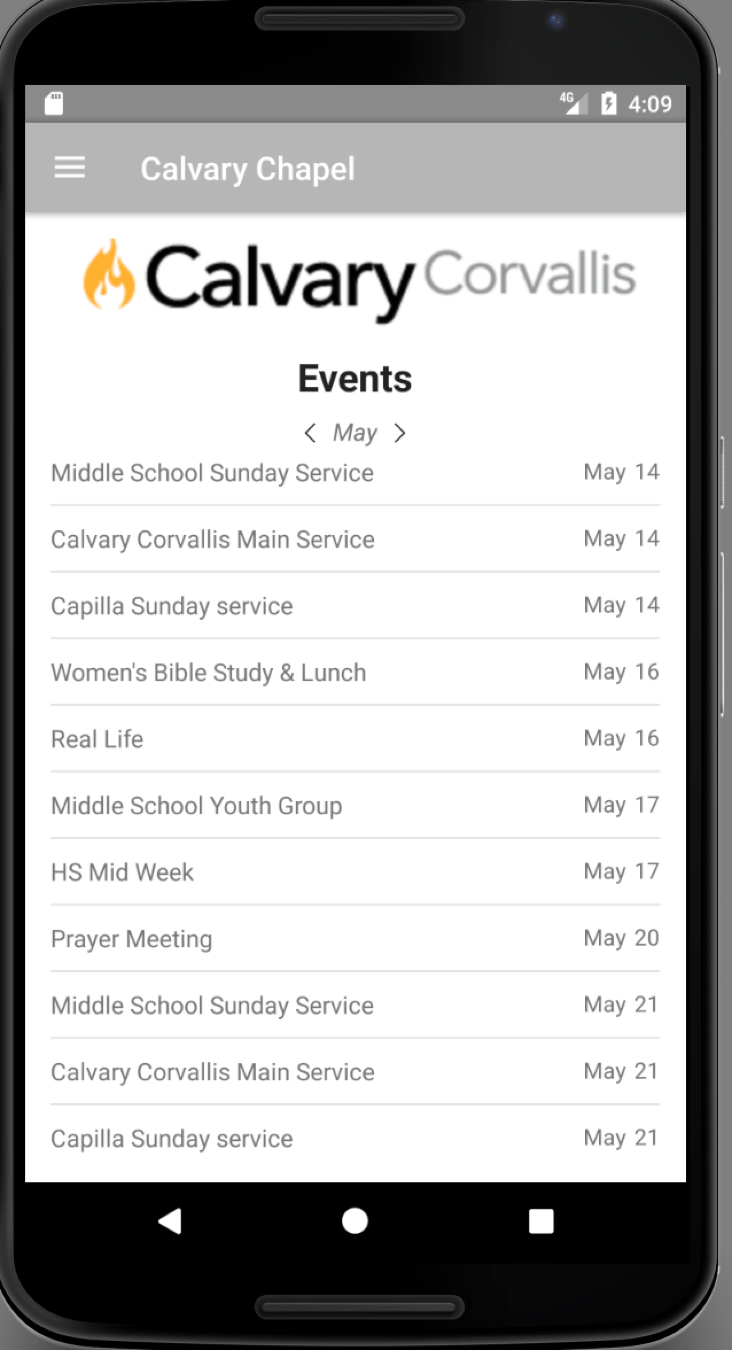
\includegraphics[width=.4\linewidth]{androidevents}
 				 \caption{A List of Events}
  				 \label{fig:sub1}
			\end{subfigure}%
			\begin{subfigure}{.5\textwidth}
		         	\centering
 				 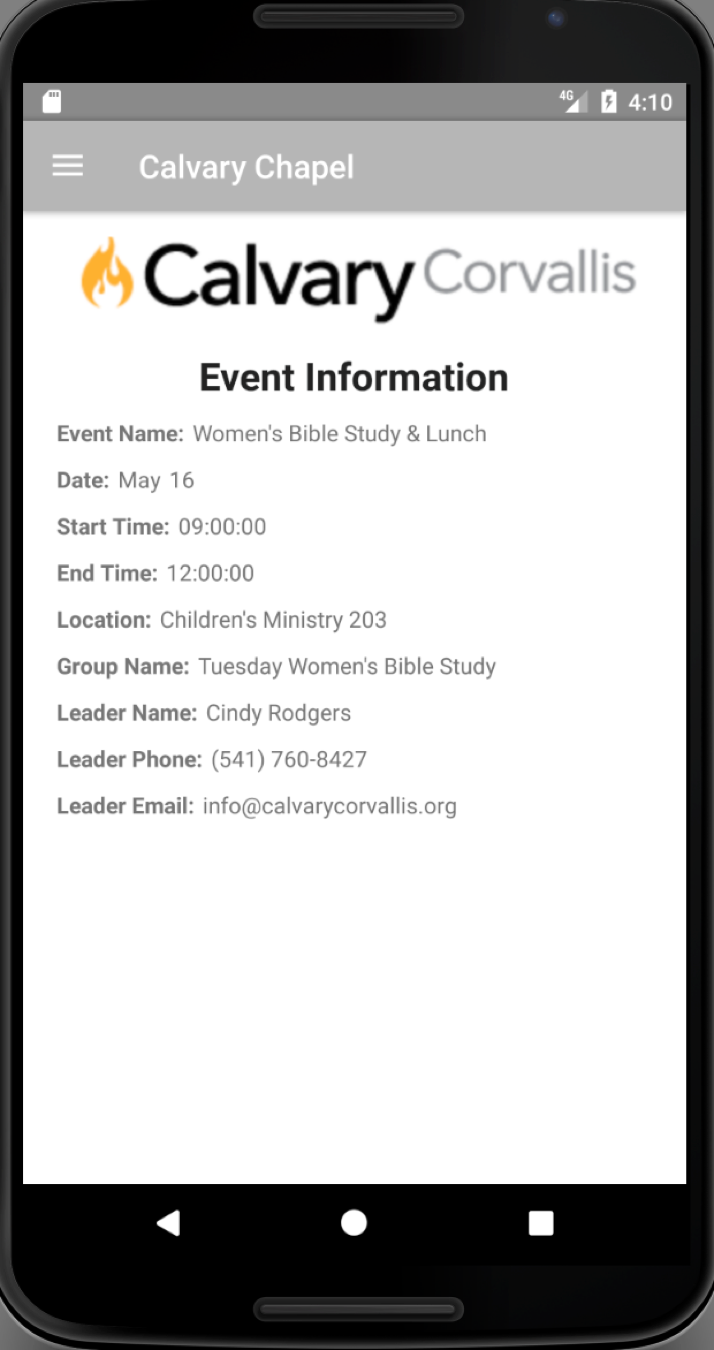
\includegraphics[width=.4\linewidth]{androiddetails}
 				 \caption{An Event Details}
 				 \label{fig:sub2}
			\end{subfigure}
			\caption{Android Event Page}
			\label{fig:event}
		\end{figure}


		\begin{figure}[H]
			\centering
			\begin{subfigure}{.5\textwidth}
 				 \centering
  				 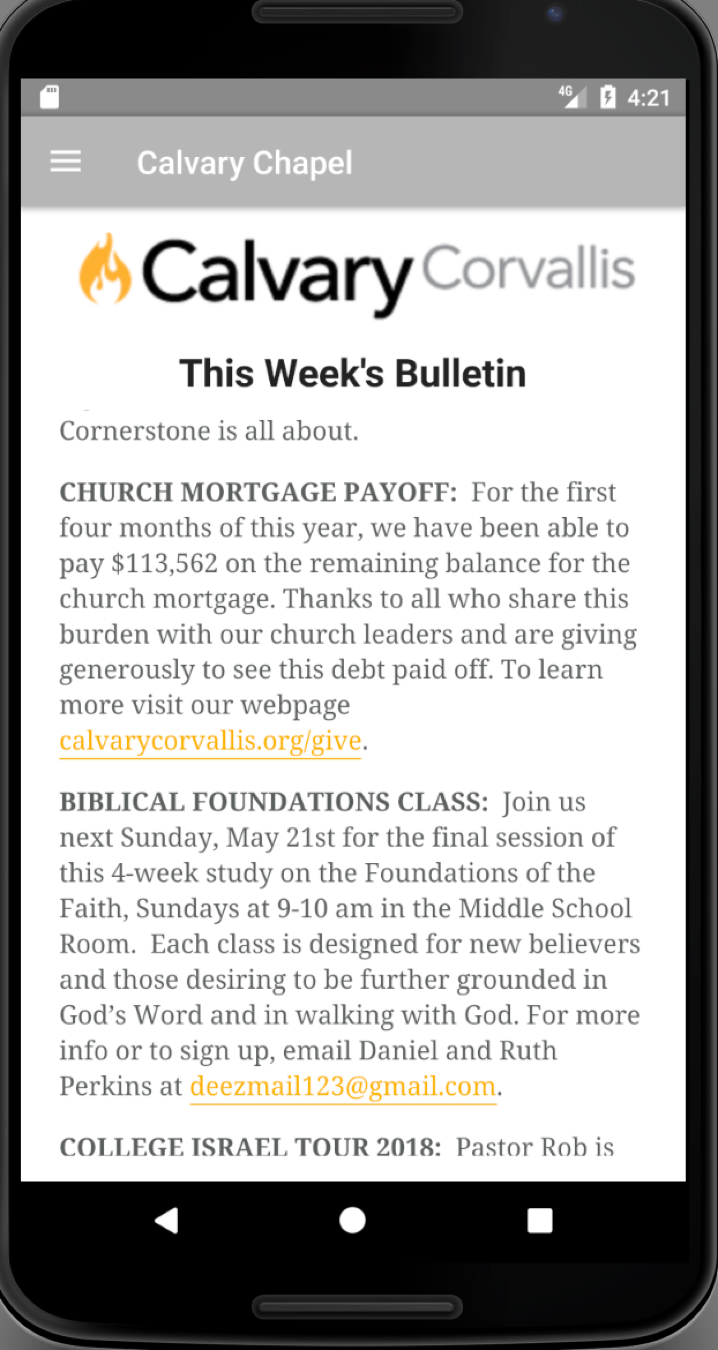
\includegraphics[width=.4\linewidth]{androidbulletin}
 				 \caption{Android}
  				 \label{fig:sub1}
			\end{subfigure}%
			\begin{subfigure}{.5\textwidth}
		         	\centering
 				 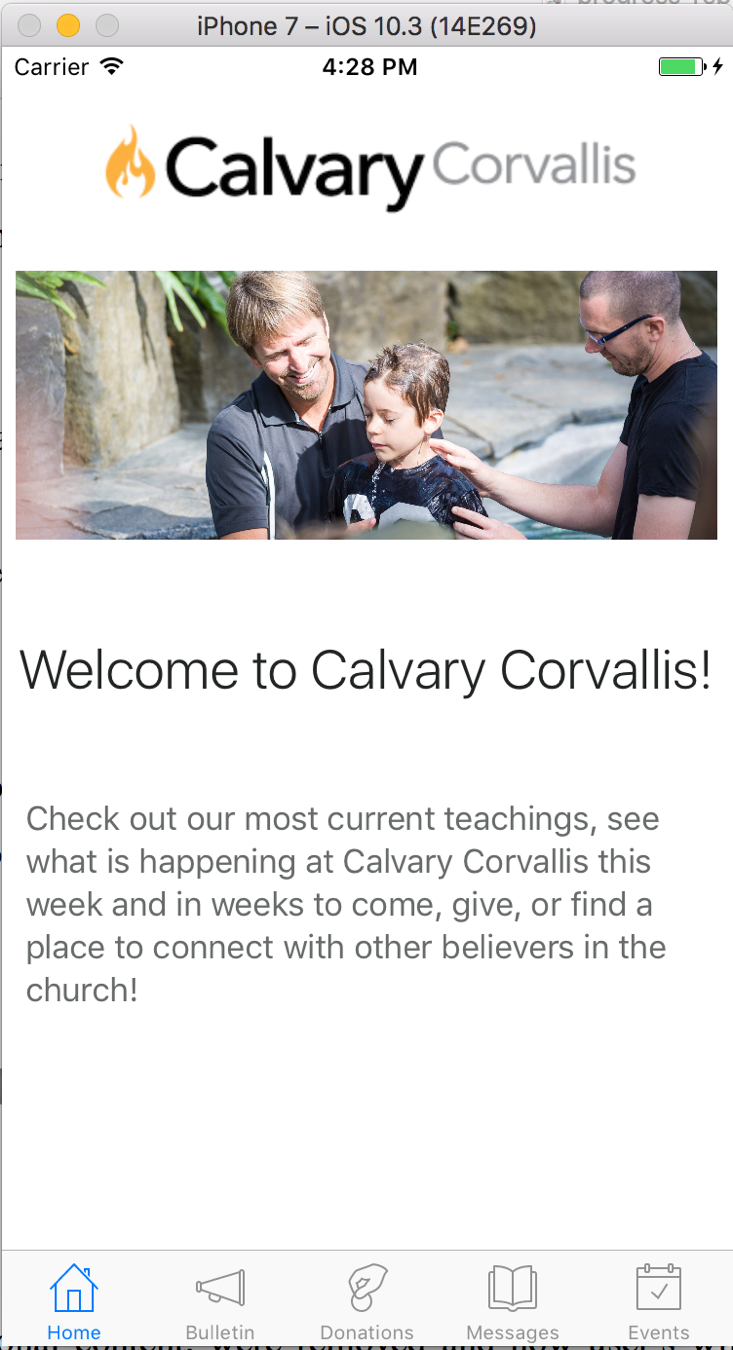
\includegraphics[width=.4\linewidth]{iosbulletin}
 				 \caption{iOS}
 				 \label{fig:sub2}
			\end{subfigure}
			\caption{Bulletin Page}
			\label{fig:bulletin}
		\end{figure}

		\begin{figure}[H]
			\centering
			\begin{subfigure}{.5\textwidth}
 				 \centering
  				 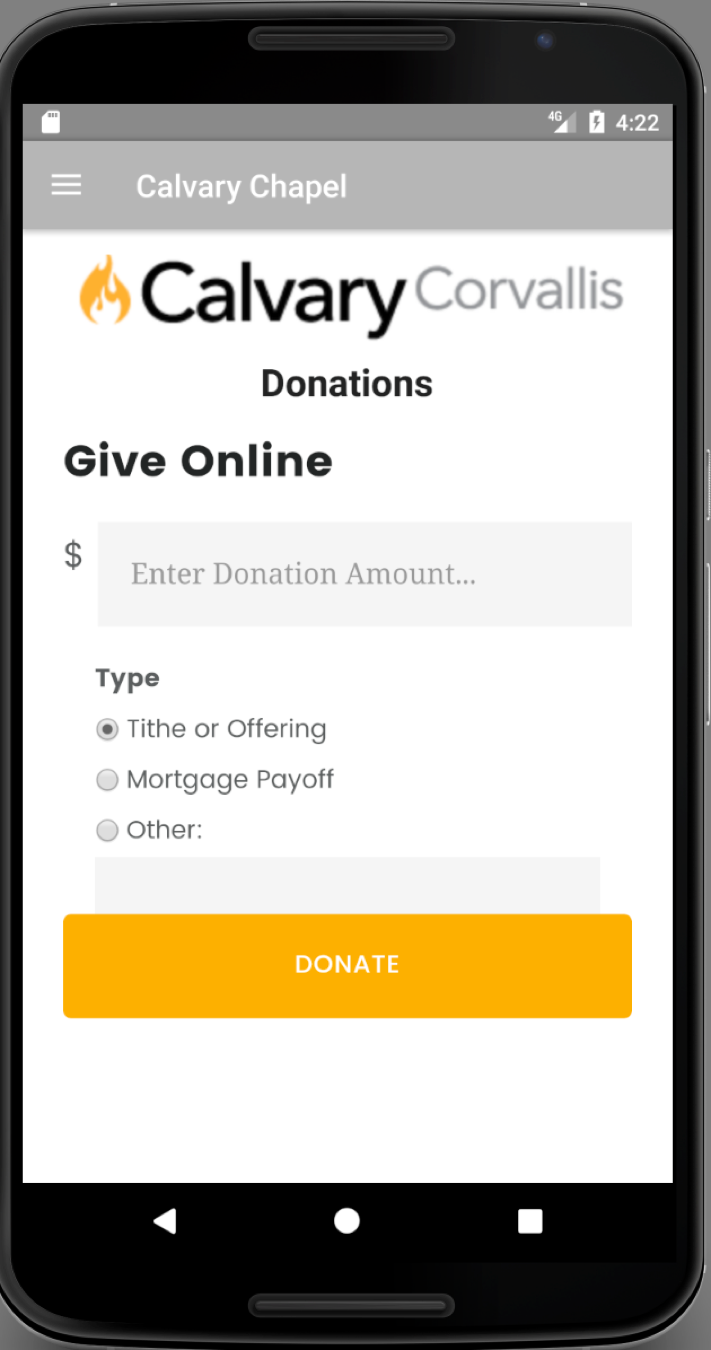
\includegraphics[width=.4\linewidth]{androiddonate}
 				 \caption{Android}
  				 \label{fig:sub1}
			\end{subfigure}%
			\begin{subfigure}{.5\textwidth}
		         	\centering
 				 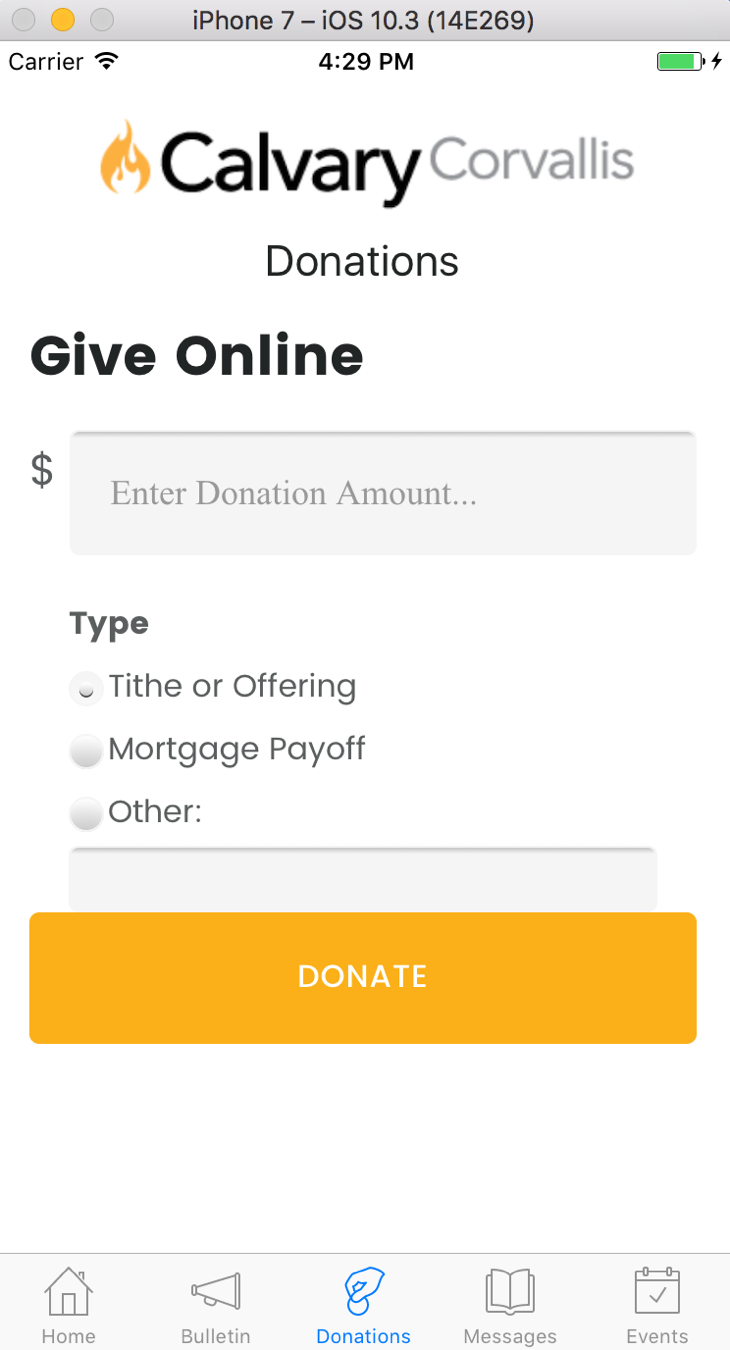
\includegraphics[width=.4\linewidth]{iosdonate}
 				 \caption{iOS}
 				 \label{fig:sub2}
			\end{subfigure}
			\caption{Donation Page}
			\label{fig:donation}
		\end{figure}

	\begin{figure}[H]
			\centering
			\begin{subfigure}{.5\textwidth}
 				 \centering
  				 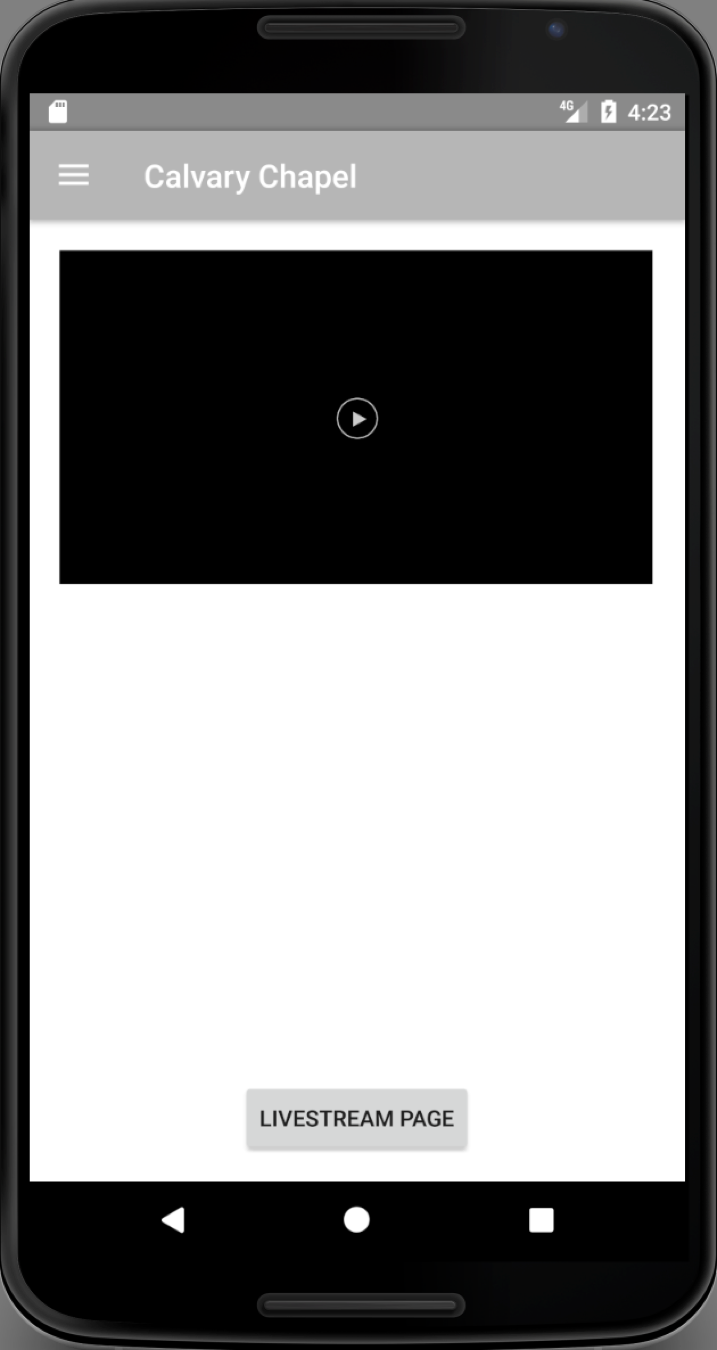
\includegraphics[width=.4\linewidth]{androidmessages}
 				 \caption{Android}
  				 \label{fig:sub1}
			\end{subfigure}%
			\begin{subfigure}{.5\textwidth}
		         	\centering
 				 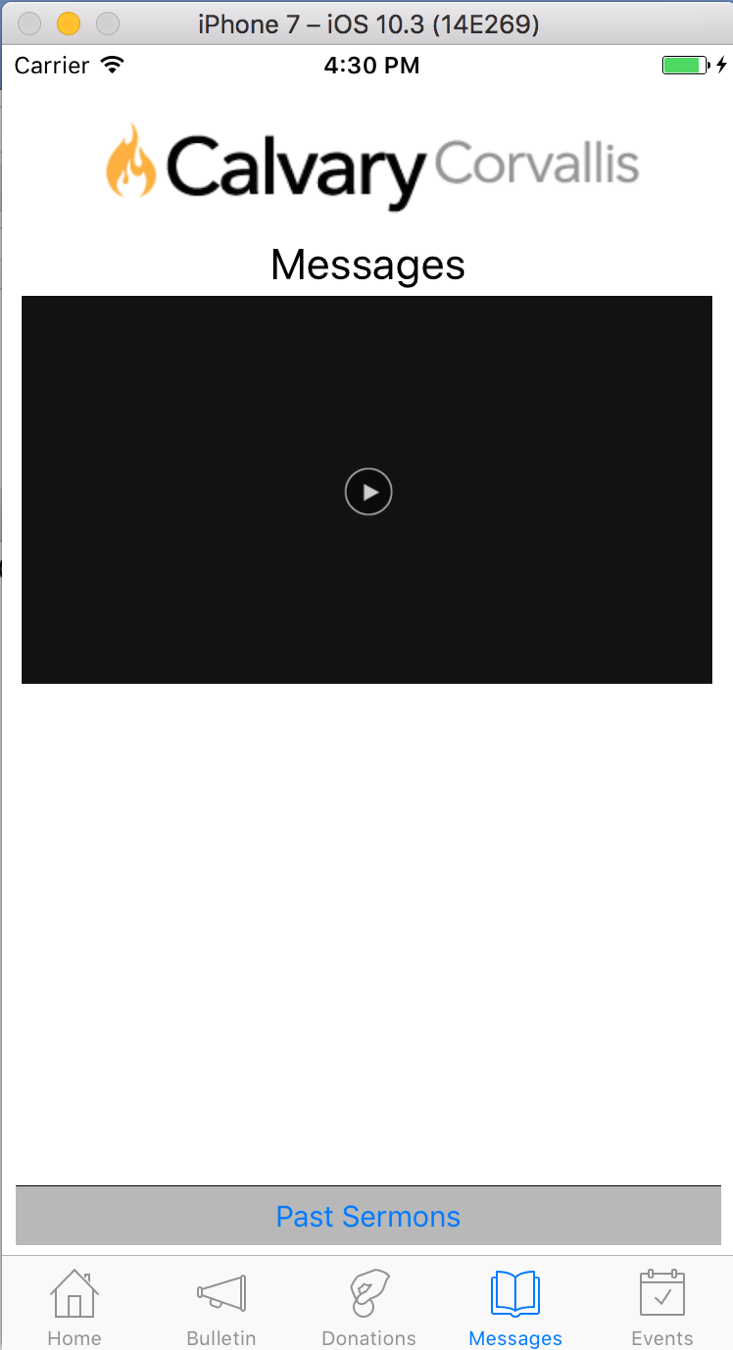
\includegraphics[width=.4\linewidth]{iosmessages}
 				 \caption{iOS}
 				 \label{fig:sub2}
			\end{subfigure}
			\caption{Messages Page}
			\label{fig:message}
		\end{figure}


\end{document}
